%%%%%%%%%%%%%%%%%%%%%%%%%%%%%%%%%%%%%%%%%
% Beamer Presentation
% Standard LaTeX Template used for creating presentation of Firebird-V Robot and other tutorials. 
% Author: Saurav Shandilya (e-Yantra Team)
% Reference: www.LaTeXTemplates.com Version 1.0 (10/11/12)
%
%%%%%%%%%%%%%%%%%%%%%%%%%%%%%%%%%%%%%%%%%

%----------------------------------------------------------------------------------------
%	PACKAGES AND THEMES
%----------------------------------------------------------------------------------------
		
\documentclass[table,10pt,red]{beamer}	% First line -- Define document class as Beamer which is used for creating presentation using Latex
\setbeamercolor{alerted text}{fg=blue} 	% Sets color of highlighted text during presentation.  
 

% The Beamer class comes with a number of default slide themes
% which change the colors and layouts of slides. Below this is a list
% of all the themes, uncomment each in turn to see what they look like.

%\usetheme{default}
%\usetheme{AnnArbor}
%\usetheme{Antibes}
%\usetheme{Bergen}
%\usetheme{Berkeley}
\usetheme{Berlin}		%used theme in present documents.
%\usetheme{Boadilla}
%\usetheme{CambridgeUS}
%\usetheme{Copenhagen}
%\usetheme{Darmstadt}
%\usetheme{Dresden}
%\usetheme{Frankfurt}
%\usetheme{Goettingen}
%\usetheme{Hannover}
%\usetheme{Ilmenau}
%\usetheme{JuanLesPins}
%\usetheme{Luebeck}
%\usetheme{Madrid}
%\usetheme{Malmoe}
%\usetheme{Marburg}
%\usetheme{Montpellier}
%\usetheme{PaloAlto}
%\usetheme{Pittsburgh}
%\usetheme{Rochester}
%\usetheme{Singapore}
%\usetheme{Szeged}
%\usetheme{Warsaw}

% As well as themes, the Beamer class has a number of color themes
% for any slide theme. Uncomment each of these in turn to see how it
% changes the colors of your current slide theme.

%\usecolortheme{albatross}
%\usecolortheme{beaver}
%\usecolortheme{beetle}
%\usecolortheme{crane}
%\usecolortheme{dolphin}
%\usecolortheme{dove}
%\usecolortheme{fly}
%\usecolortheme{lily}
%\usecolortheme{orchid}
%\usecolortheme{rose}
%\usecolortheme{seagull}
%\usecolortheme{seahorse}
%\usecolortheme{whale}
%\usecolortheme{wolverine}

%\setbeamertemplate{footline} % To remove the footer line in all slides uncomment this line
%\setbeamertemplate{footline}[page number] % To replace the footer line in all slides with a simple slide count uncomment this line

%\setbeamertemplate{navigation symbols}{} % To remove the navigation symbols from the bottom of all slides uncomment this line
%}

%------------------------------------------------------------------------------------------
%	\usepackage is required for including various features like images, table, references etc.
%	Packages must be installed before using. These can be istalled through package manager. 
%   Various packages have dependencies and for using such packages all dependent packages must be used. 
%-----------------------------------------------------------------------------------------
\usepackage{beamerthemeshadow} % theme shadow for visual 
\usepackage{beamerthemesplit} % Creates minipage (for showing multiple images and text) on same page  
\usepackage{graphicx} % Allows including images
\usepackage{booktabs} % Allows the use of \toprule, \midrule and \bottomrule in tables
\usepackage{xcolor}
\usepackage{booktabs,array}
\usepackage{listings}
\usepackage{hyperref}	% Required for including hyperlink in document
\usepackage{verbatim,moreverb} % Required for including code snippet.
\usepackage{colortbl}
\usepackage{multirow}	% Required for creating multiple row tables
\usepackage{tikz}		% Required for drawing shapes such as circles, arrowed line, etc. 
\usetikzlibrary{arrows}

% logo
\logo{
\includegraphics[height=1cm]{iitblogo.pdf}} % includes logo at bottom of all slides 

%----------------------------------------------------------------------------------------
%	TITLE PAGE
%----------------------------------------------------------------------------------------
% sf family, bold font
\sffamily \bfseries
% content inside [] appears at bottom of all page. content inside {} appears on first page as title. double backslash means line change 
\title
[
	RFID Module Interface	% bottom of all page
	\hspace{0.5cm}
	\insertframenumber/\inserttotalframenumber
]
{
Interfacing RFID Module with FireBird V 
}

\author
[
	www.e-yantra.org 	%Name at bottom of all page 
]
% author name on title slide
{  \\
  Embedded Real-Time Systems Lab\\
  Indian Institute of Technology-Bombay \\
}
\date
{
IIT Bombay \\ {\today}	%\today picks system date on title slide
}

\begin{document} % IN LATEX ALL DOCUMENT/REPORT/PRESENTATION STARTS WITH \begin{document} AND ENDS WITH \end{document}

\begin{frame}	% FRAME MEANS SLIDE. \begin{frame} STARTS THE SLIDE AND \end{frame} ENDS THE SLIDE
	\titlepage % Print the title page as the first slide
\end{frame}

% START OF SECOND SLIDE
\begin{frame}
	\frametitle{Agenda for Discussion} % Table of contents slide, comment this block out to remove it
	\tableofcontents % Throughout your presentation, if you choose to use \section{} and \subsection{} commands, these will automatically be printed on this slide as an overview of your presentation
\end{frame}

%----------------------------------------------------------------------------------------
%	PRESENTATION SLIDES
%----------------------------------------------------------------------------------------

%------------------------------------------------
\section{Introduction to RFID Module} % Sections can be created in order to organize your presentation into discrete blocks, all sections and subsections are automatically printed in the table of contents as an overview of the talk
%------------------------------------------------


% Start of Third slide
\begin{frame}
	\frametitle{What is an RFID ??}
 		\begin{enumerate}[$\checkmark$]
 				\item <+-|alert@+> Radio-frequency identification (RFID) is the wireless non-contact use of radio-frequency electromagnetic fields to transfer data. 
 				 
 				
 				\item <+-|alert@+> The main purpose of using RFID is to automatically identify and track the active and passive tags attached to various objects in our daily life.
 				
 				\item <+-|alert@+> RFID tags are an improvement over bar codes because the tags have read and write capabilities. Data stored on RFID tags can be changed, updated and locked.  
 				
 				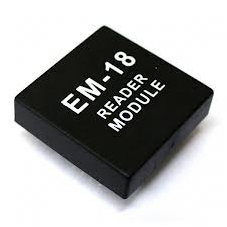
\includegraphics[scale=0.5]{rfid1}
 			\hspace{1in}	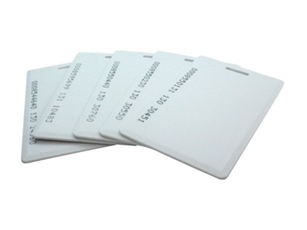
\includegraphics[scale=0.75]{rfidtag}
 				
 		\end{enumerate}
\end{frame}

%------------------------------------------------
\section{EM-18 RFID Reader Module}
% Start of fourth slide
\subsection{EM-18 RFID Reader  Module} % A subsection can be created just before a set of slides with a common theme to further break down your presentation into chunks
\begin{frame}
	\frametitle{EM 18 RFID Reader}
	\begin{minipage}[c]{0.2\textwidth}
				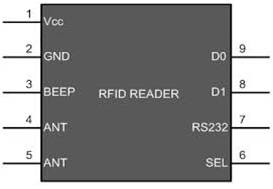
\includegraphics[width=\linewidth]{rfidpin}
			\end{minipage}
		\pause
		\hfill
			\begin{minipage}[c]{0.75\textwidth}
				\begin{enumerate}
					\item <+-|alert@+> \small EM-18 operates on $+5V$ power supply. 
					\item <+-|alert@+>Read frequency of the reader is 125kHz
					\item <+-|alert@+>maximum read range is 10 cm
					
					\item <+-|alert@+> The serial transmission rate is 9600bps, TTL and RS232 output
				
					
				\end{enumerate}
			\end{minipage}   

\end{frame}




\subsection{Continued...} % A subsection can be created just before a set of slides with a common theme to further break down your presentation into chunks
\begin{frame}
	\frametitle{ EM 18 RFID Reader Continued...}
	\begin{minipage}[c]{0.2\textwidth}
				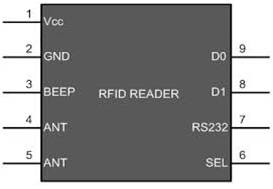
\includegraphics[width=\linewidth]{rfidpin}
			\end{minipage}
		\pause
		\hfill
			\begin{minipage}[c]{0.75\textwidth}
				\begin{enumerate}
					\item <+-|alert@+> Pin 1 and 2: These are supply and ground pins
					\item <+-|alert@+> Pin 3: The Beep pin is the output pin which provides series of pulses which could be connected to an led or a buzzer for the read indication
					\item <+-|alert@+> Pin 4 and 5: These two are antenna pins which are left unconnected.
					\item <+-|alert@+> Pin 6: SEL Pin is pulled high to get RS232 output. If the Pin is held low then data is received from DO and D1 pins.
					\item <+-|alert@+> Pin 7: The serial output is taken from this pin in RS232 format
					\item <+-|alert@+> Pin 8 and 9: These Data signal Pins used to output the data in 26 bit Wiegand format 
				
					
				\end{enumerate}
			\end{minipage}   

\end{frame}





\section{Interfacing RFID Module On FireBird V} % A subsection can be created just before a set of slides with a common theme to further break down your presentation into chunks
\subsection{Application circuit of RFID Module}
\begin{frame}
	\frametitle{Application circuit}

				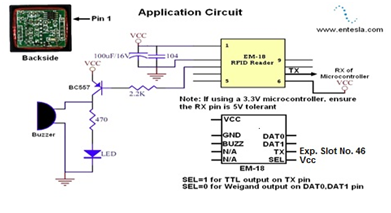
\includegraphics[scale=1]{rfidapp}
		
\end{frame}


\subsection{Interfacing RFID Module on FireBird V}
\begin{frame}
	\frametitle{Application circuit}

				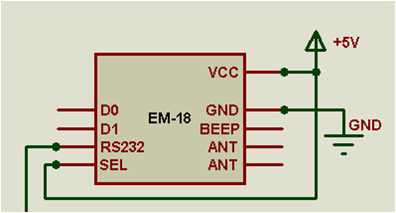
\includegraphics[scale=0.25]{rfidckt}
				\hspace{0.2in}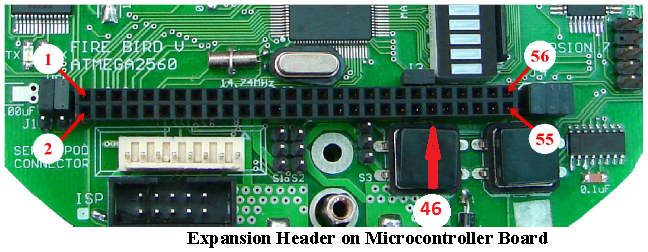
\includegraphics[scale=0.29]{exp}
				
			\hspace{0.06in}	$\downarrow$
		
			To RX pin of MCU i.e., Pin 46\\on expansion slot
		
\end{frame}



\section{RFID Module Testing} % A subsection can be created just before a set of slides with a common theme to further break down your presentation into chunks

\subsection{Connecting RFID Module to USB to Serial Converter} % A subsection can be created just before a set of slides with a common theme to further break down your presentation into chunks
\begin{frame}
	\frametitle{USB to Serial Converter}
	\begin{minipage}[c]{0.2\textwidth}
				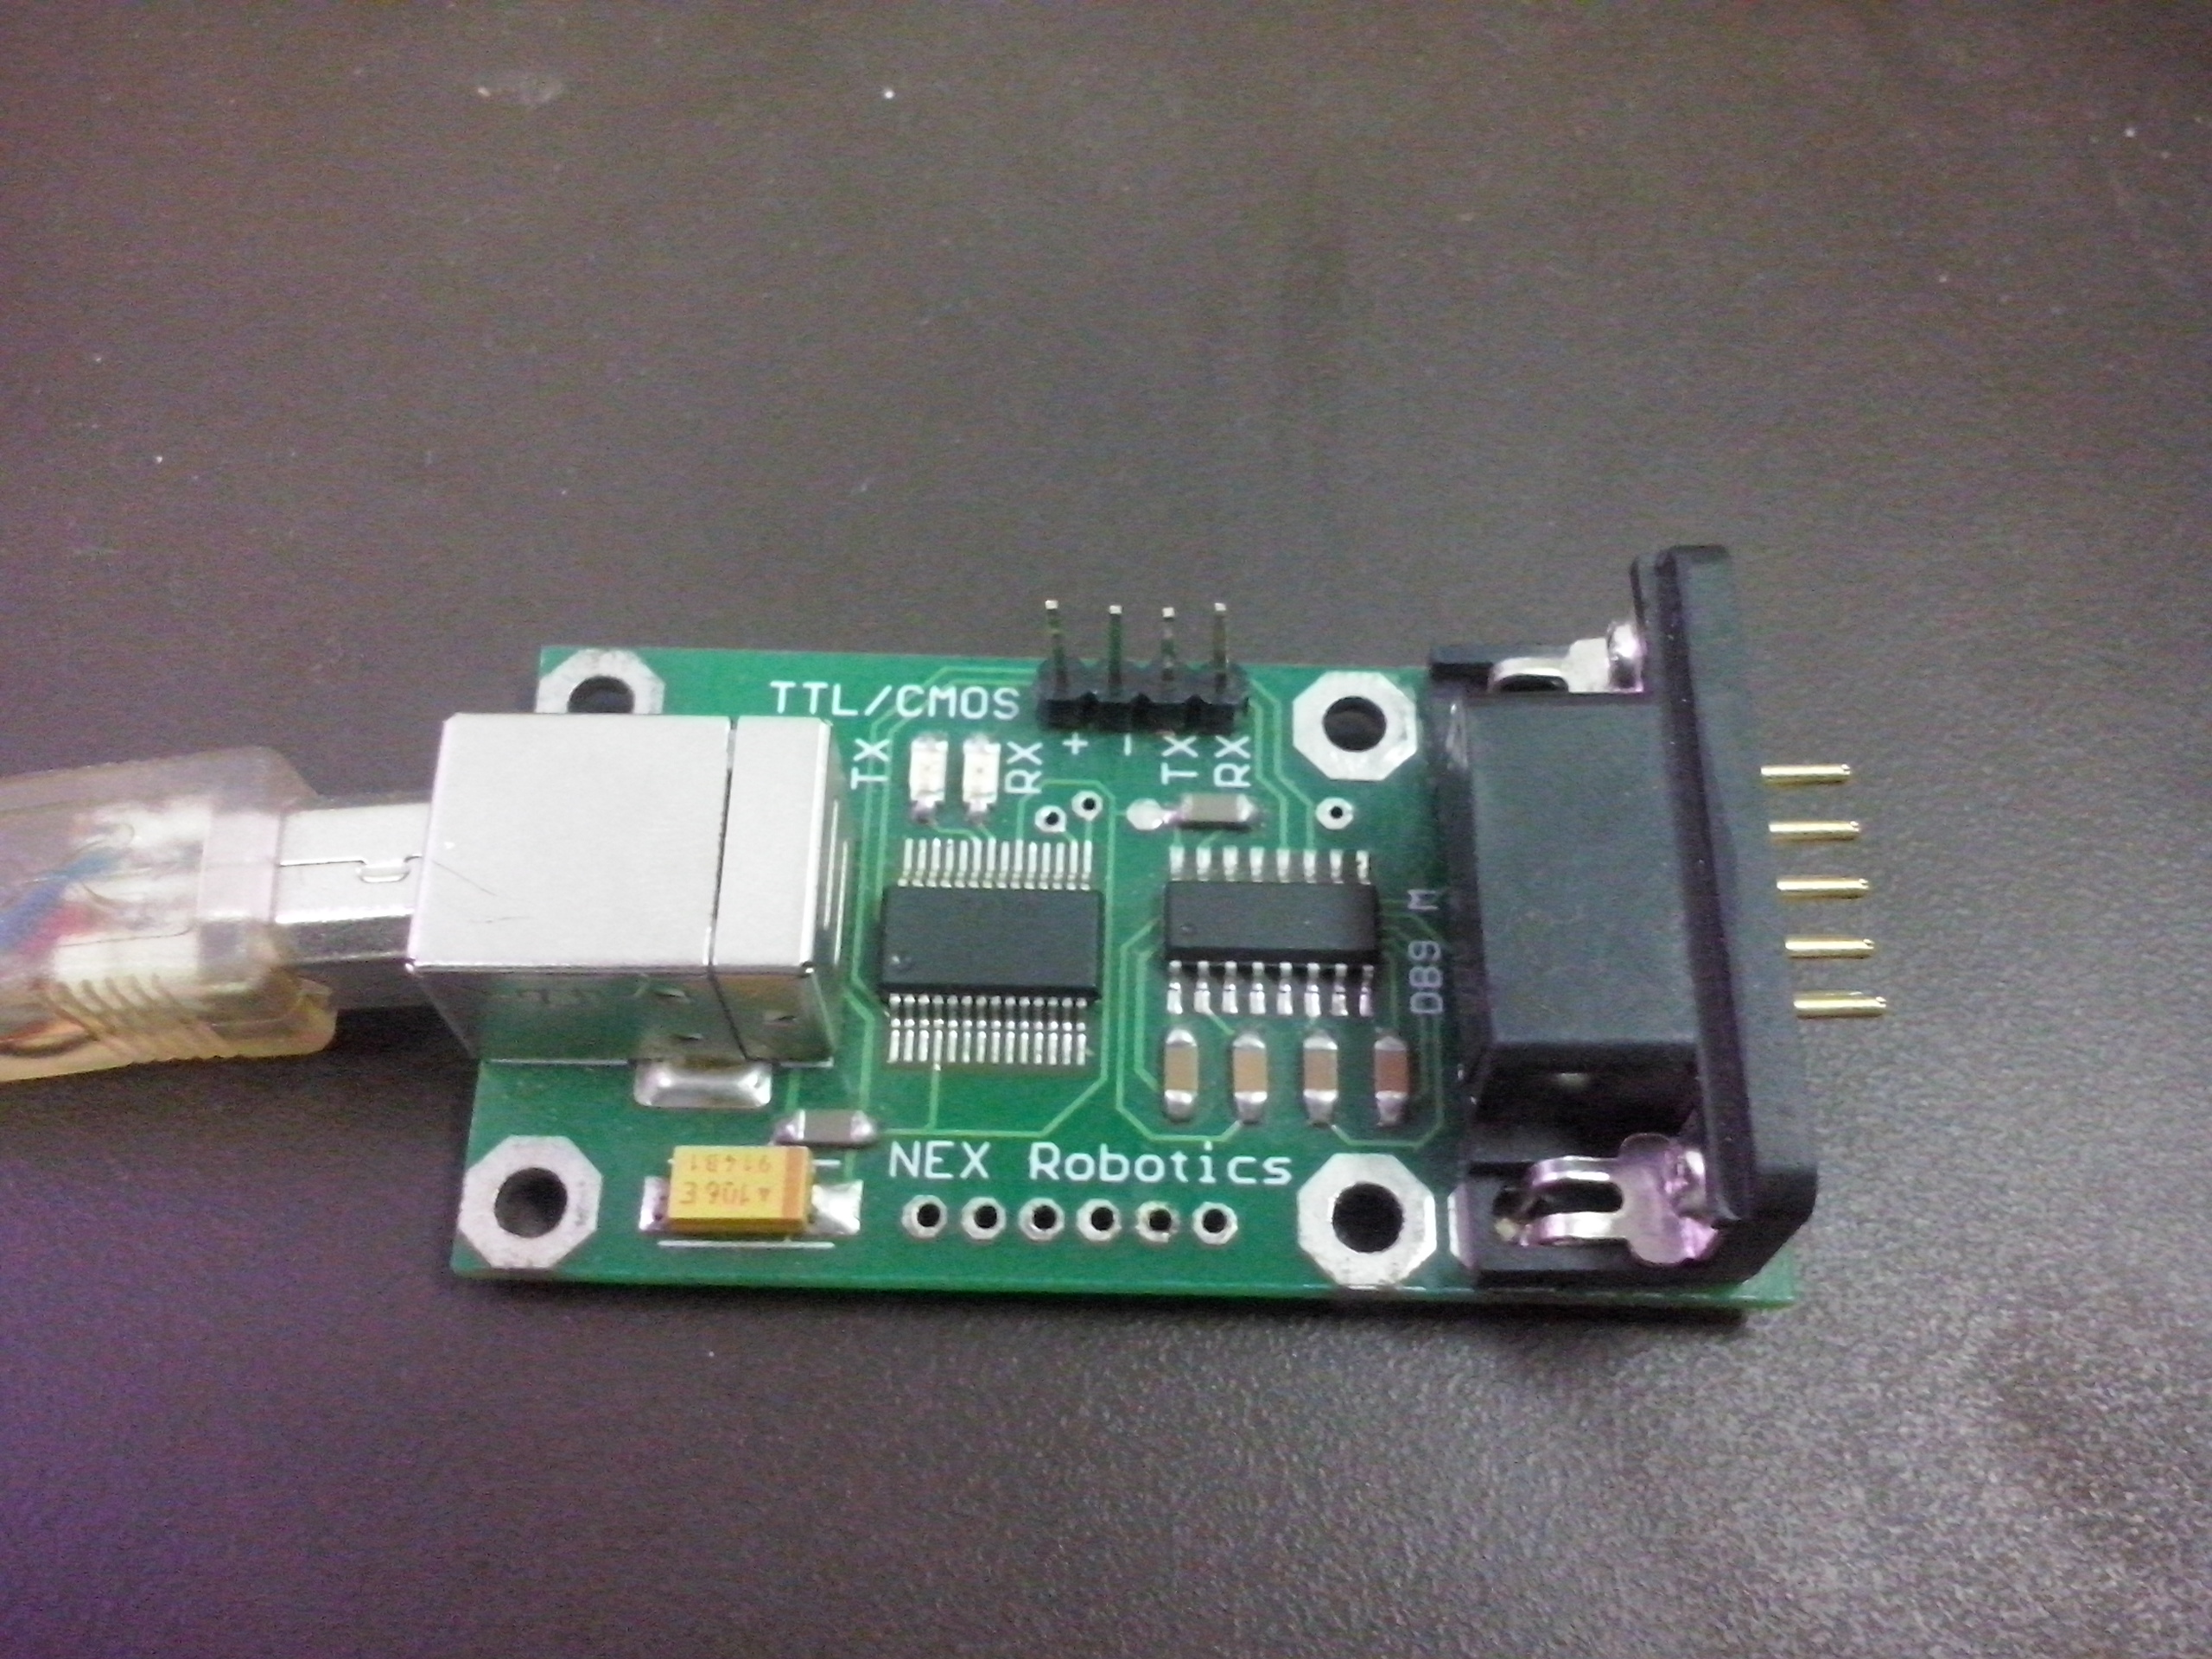
\includegraphics[width=\linewidth]{usb1}\\\\
				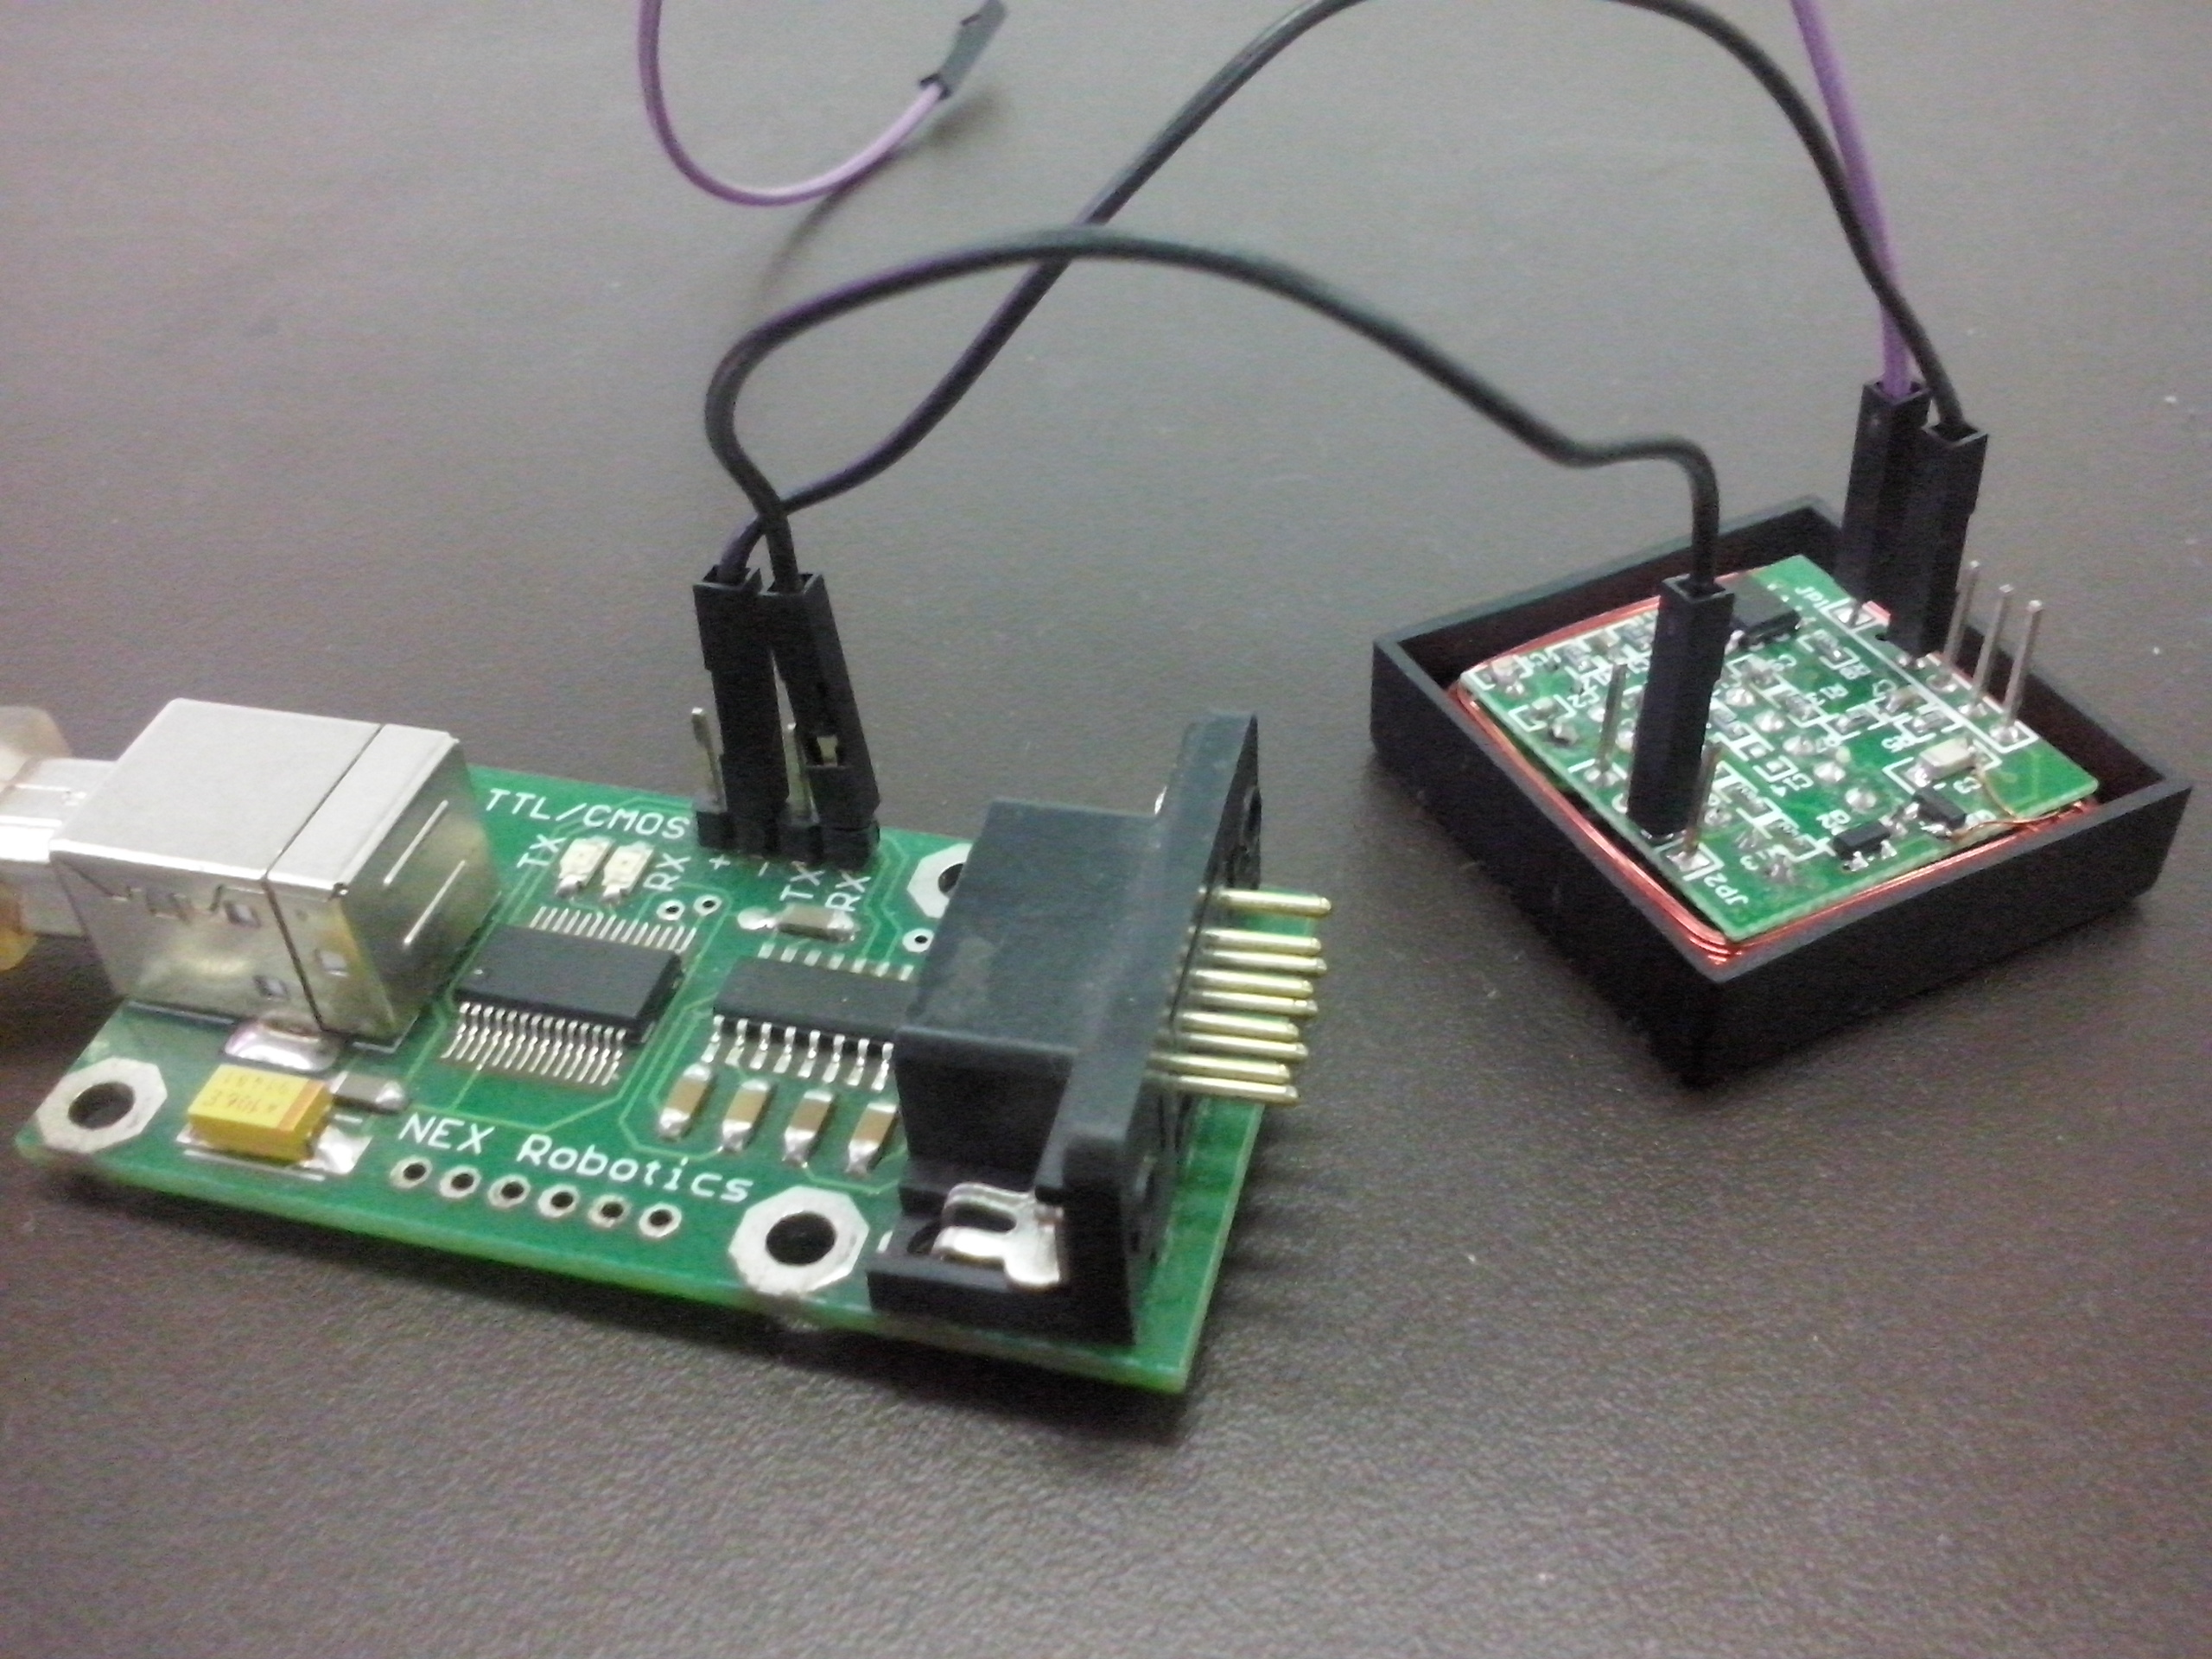
\includegraphics[width=\linewidth]{usb2}\\\\
			\end{minipage}
		\pause
		\hfill
			\begin{minipage}[c]{0.75\textwidth}
				\begin{enumerate}
					\item The figure shows the USB to Serial converter
					\item The figure shows the connections to be made for serial transmission
					\item connect the common ground - pin of the converter
					\item VCC Pin of the Converter need not be connected
					\item The RS232 output pin is connected to RX pin of the Converter
				
					
				\end{enumerate}
			\end{minipage}   

\end{frame}

\subsection{Sample output as seen on serial terminal}
\begin{frame}
	\frametitle{Serial terminal}
	\begin{minipage}[c]{0.2\textwidth}
				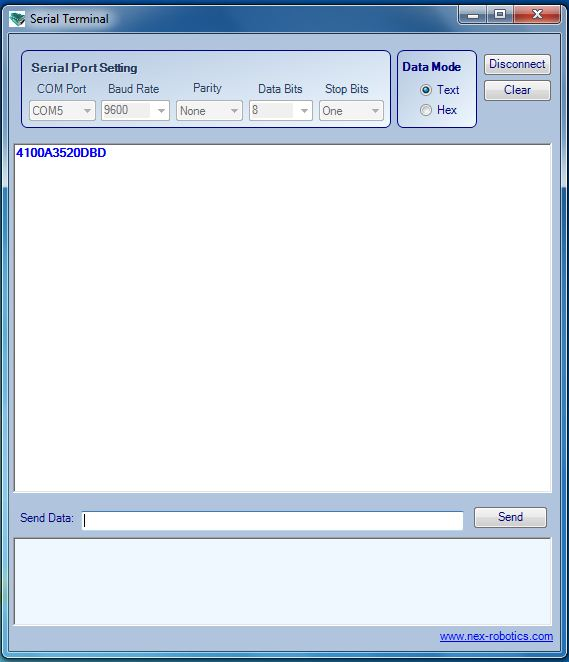
\includegraphics[width=\linewidth]{st}
				
			\end{minipage}
			\hfill
			\begin{minipage}[c]{0.75\textwidth}
			\begin{enumerate}\small
			\item 1. Open the serial terminal software
			\item 2. Set the COM port for the device
			\item 3. Set the baud rate to 9600
			\item 4. Set the number of start bits, stop bits and parity bits
			\item 5. Change the Data mode to Text
			\end{enumerate}
			\end{minipage}
			

\end{frame}

\subsection{Sample output on LCD screen}
\begin{frame}
	\frametitle{Sample output on LCD screen of FBV}
			\begin{center}	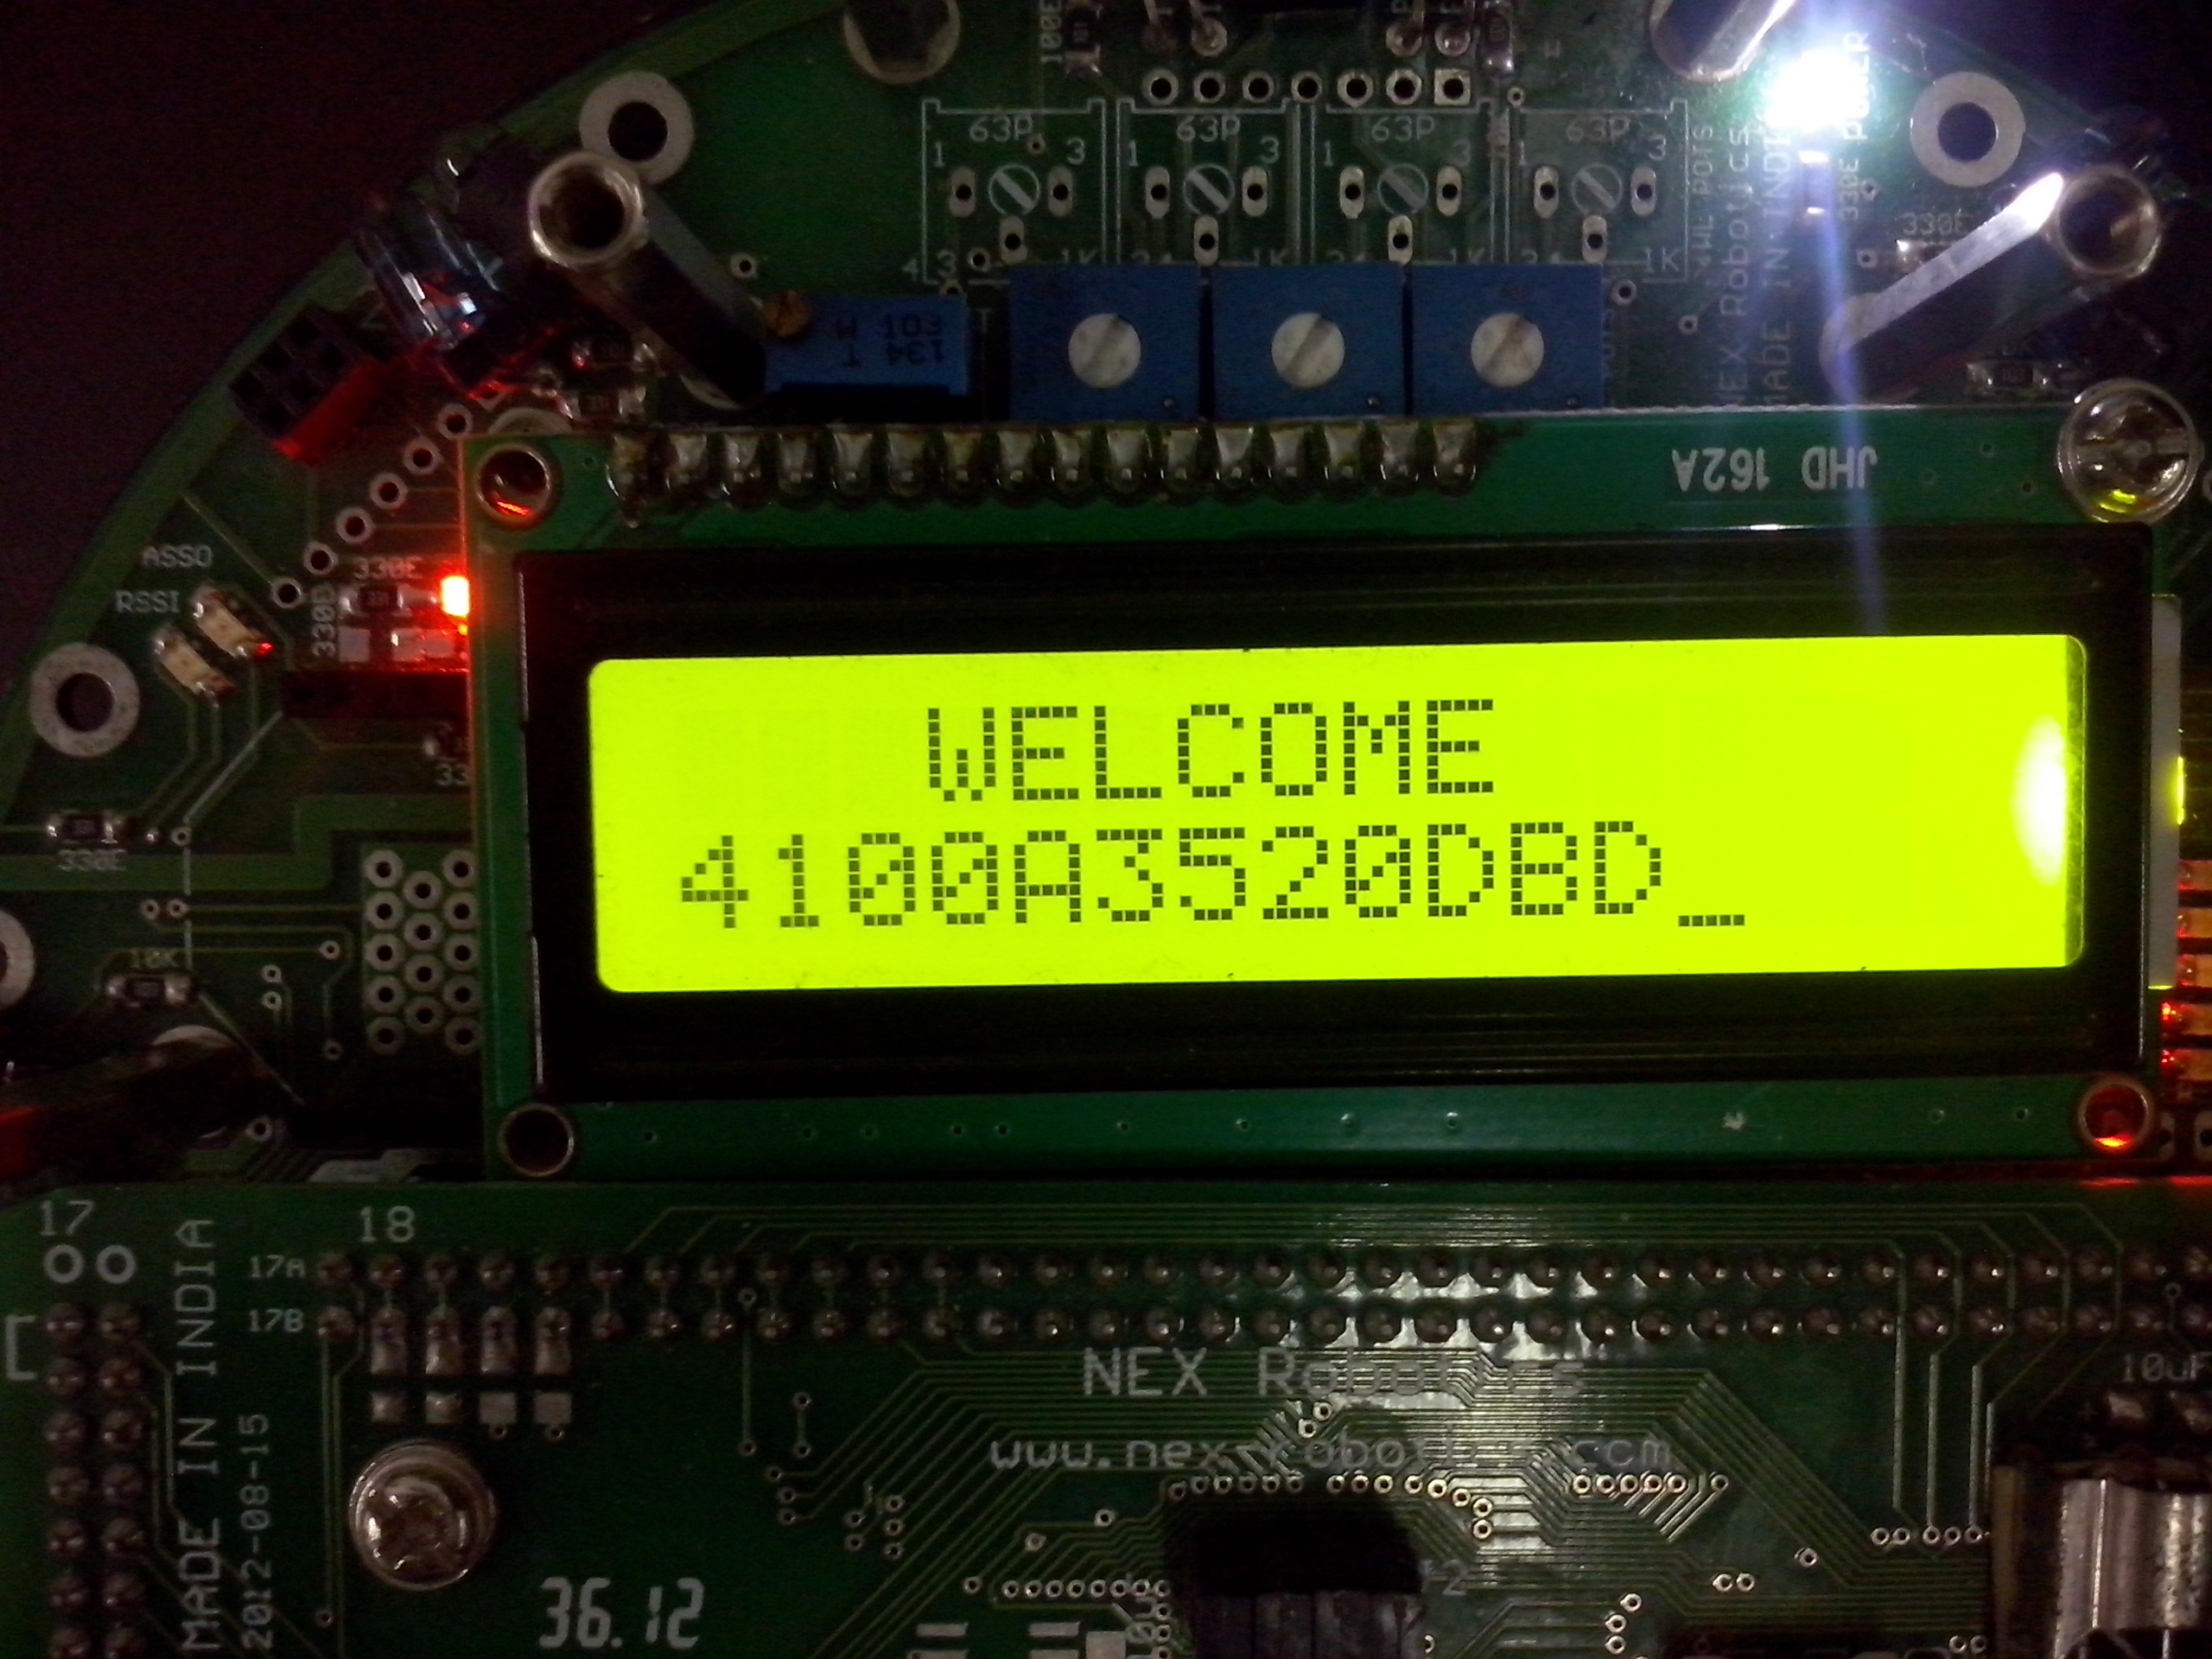
\includegraphics[scale=0.08]{detected}
\end{center}

\end{frame}

\section{C Code} % Sections can be created in order to organize your presentation into discrete blocks, all sections and subsections are automatically printed in the table of contents as an overview of the talk
%------------------------------------------------


% Start of Third slide
\begin{frame}
	\frametitle{C Code}
 		\begin{center}
 		\Huge C Code
 		\end{center}
\end{frame}




\end{document} 